\section{The Four Classical HMM Algorithms: Pseudocode and Toy Example}
\label{sec:algorithms}

Each algorithm below is implemented from scratch in NumPy (module
\texttt{oilbn.models.hmm}, class \texttt{HiddenMarkovRegimeModel}), in
log-space throughout for numerical stability, and demonstrated on a
shared toy model before being applied to real WTI/Brent data in
Section~\ref{sec:regime-process}. The toy model has two well-separated states
($\mu_0=-5$, $\mu_1=+5$, $\sigma_0=\sigma_1=1$, self-transition
probability $0.9$), so every algorithm's output can be sanity-checked by
eye.

\subsection{Forward and Backward (Evaluation) --- Student A}

The Forward algorithm answers "how likely is this observed sequence
under the model?" by recursively accumulating, for every state $i$ and
time $t$, the joint probability of the observations seen so far
\emph{and} being in state $i$ at time $t$. The Backward algorithm
computes the complementary quantity -- the probability of everything
\emph{after} time $t$, given state $i$ at time $t$ -- and the two
together give the posterior state-occupation probabilities
$\gamma_t(i)$ used by Baum-Welch.

\begin{algorithm}[H]
\caption{Forward algorithm (log-space)}
\begin{algorithmic}[1]
\Require Observations $x_{1:T}$; model $\lambda = (\pi, A, \{\mu_k,\sigma_k^2\})$
\Ensure $\log\alpha_t(i)$ for all $t,i$; total log-likelihood $\log p(x_{1:T}\mid\lambda)$
\For{each state $i$}
  \State $\log\alpha_1(i) \gets \log\pi_i + \log\mathcal{N}(x_1;\mu_i,\sigma_i^2)$
\EndFor
\For{$t = 2, \ldots, T$}
  \For{each state $j$}
    \State $\log\alpha_t(j) \gets \mathrm{logsumexp}_i\bigl(\log\alpha_{t-1}(i) + \log A_{ij}\bigr) + \log\mathcal{N}(x_t;\mu_j,\sigma_j^2)$
  \EndFor
\EndFor
\State \Return $\{\log\alpha_t(i)\}$, $\mathrm{logsumexp}_i\bigl(\log\alpha_T(i)\bigr)$
\end{algorithmic}
\end{algorithm}

\begin{algorithm}[H]
\caption{Backward algorithm (log-space)}
\begin{algorithmic}[1]
\Require Observations $x_{1:T}$; model $\lambda$
\Ensure $\log\beta_t(i)$ for all $t,i$
\For{each state $i$}
  \State $\log\beta_T(i) \gets 0$
\EndFor
\For{$t = T-1, \ldots, 1$}
  \For{each state $i$}
    \State $\log\beta_t(i) \gets \mathrm{logsumexp}_j\bigl(\log A_{ij} + \log\mathcal{N}(x_{t+1};\mu_j,\sigma_j^2) + \log\beta_{t+1}(j)\bigr)$
  \EndFor
\EndFor
\State \Return $\{\log\beta_t(i)\}$
\end{algorithmic}
\end{algorithm}

\textbf{Toy-example check.} On the 6-observation sequence $(-5.1, -4.9,
-5.0, 5.0, 4.9, 5.1)$, the Forward algorithm returns $\log
p(O\mid\lambda) = -8.9508$; the posterior state-occupation probabilities
$\gamma_t(i) = \exp(\log\alpha_t(i) + \log\beta_t(i) - \log
p(O\mid\lambda))$ sum to exactly $1.0$ at every one of the $T=6$
timesteps, confirming the Forward-Backward recursions are implemented
consistently with each other.

\subsection{Viterbi (Decoding) --- Student B}

Viterbi finds the single most likely \emph{complete} state path, rather
than the per-timestep marginal regime probability -- the natural choice
for assigning one discrete regime label per day, which Section
\ref{sec:regime-process} then resamples to monthly frequency for the Bayesian
network.

\begin{algorithm}[H]
\caption{Viterbi algorithm (log-space)}
\begin{algorithmic}[1]
\Require Observations $x_{1:T}$; model $\lambda$
\Ensure Most likely state path $q_{1:T}^\ast$
\For{each state $i$}
  \State $\delta_1(i) \gets \log\pi_i + \log\mathcal{N}(x_1;\mu_i,\sigma_i^2)$
\EndFor
\For{$t = 2, \ldots, T$}
  \For{each state $j$}
    \State $\delta_t(j) \gets \max_i\bigl(\delta_{t-1}(i) + \log A_{ij}\bigr) + \log\mathcal{N}(x_t;\mu_j,\sigma_j^2)$
    \State $\psi_t(j) \gets \arg\max_i\bigl(\delta_{t-1}(i) + \log A_{ij}\bigr)$ \Comment{backpointer}
  \EndFor
\EndFor
\State $q_T^\ast \gets \arg\max_i \delta_T(i)$
\For{$t = T-1, \ldots, 1$}
  \State $q_t^\ast \gets \psi_{t+1}(q_{t+1}^\ast)$ \Comment{backtrack}
\EndFor
\State \Return $q_{1:T}^\ast$
\end{algorithmic}
\end{algorithm}

\textbf{Toy-example check.} On the same 6-observation sequence, Viterbi
decodes the path $(0,0,0,1,1,1)$ -- exactly the generating regime
pattern implied by the hand-picked observation values -- with
$\log P(q^\ast, O \mid \lambda) = -8.9508$, matching the Forward
algorithm's total log-likelihood to 4 decimal places (expected on an
unambiguous sequence like this one, where the single best path
essentially accounts for all of the probability mass).

\subsection{Baum-Welch (Training) --- Student C}

Baum-Welch is Expectation-Maximization applied to the HMM
(Section~\ref{sec:hmm-definition}): each iteration re-estimates every
parameter from the current posterior state-occupation ($\gamma$) and
state-transition ($\xi$) probabilities, computed via one Forward and one
Backward pass.

\begin{algorithm}[H]
\caption{Baum-Welch (one EM iteration)}
\begin{algorithmic}[1]
\Require Observations $x_{1:T}$; current model $\lambda^{(n)}$
\Ensure Updated model $\lambda^{(n+1)}$
\State \textbf{E-step:} run Forward and Backward (Algorithms 1--2) to get $\log\alpha,\log\beta,\log p(x_{1:T}\mid\lambda^{(n)})$
\State $\gamma_t(i) \gets \exp\bigl(\log\alpha_t(i)+\log\beta_t(i)-\log p(x_{1:T}\mid\lambda^{(n)})\bigr)$ for all $t,i$
\State $\xi_t(i,j) \gets \exp\bigl(\log\alpha_t(i)+\log A_{ij}+\log\mathcal{N}(x_{t+1};\mu_j,\sigma_j^2)+\log\beta_{t+1}(j)-\log p(x_{1:T}\mid\lambda^{(n)})\bigr)$
\State \textbf{M-step:}
\State $\pi_i \gets \gamma_1(i)$
\State $A_{ij} \gets \sum_t \xi_t(i,j) \big/ \sum_t \gamma_t(i)$
\State $\mu_i \gets \sum_t \gamma_t(i)\, x_t \big/ \sum_t \gamma_t(i)$
\State $\sigma_i^2 \gets \sum_t \gamma_t(i)\,(x_t-\mu_i)^2 \big/ \sum_t \gamma_t(i)$
\State \Return $\lambda^{(n+1)} = (\pi, A, \{\mu_i,\sigma_i^2\})$
\end{algorithmic}
\end{algorithm}

\textbf{Toy-example check.} Starting from a deliberately noisy
initialization and training on $1{,}000$ observations simulated from the
toy model, Baum-Welch converges in 5 iterations (improvement
$<10^{-6}$), recovers means $(-5.05, 4.89)$ against true values $(-5,
5)$ and the exact true self-transition probability $(0.9, 0.9)$, and --
critically -- the total log-likelihood increases monotonically at
every one of the 5 iterations (Figure~\ref{fig:baum-welch-convergence}),
the defining guarantee of EM.

\begin{figure}[H]
  \centering
  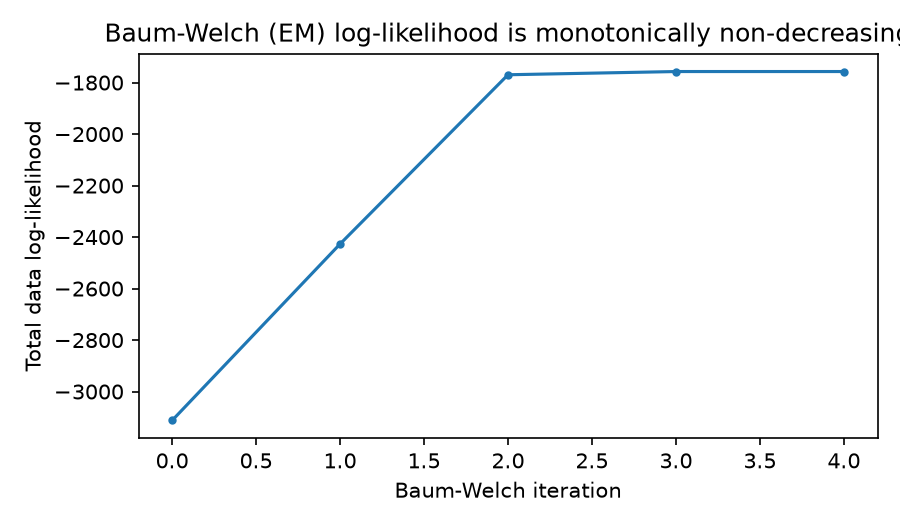
\includegraphics[width=0.75\textwidth]{figures/baum_welch_toy_convergence.png}
  \caption{Baum-Welch log-likelihood across EM iterations on the toy
    model: monotonically non-decreasing, as EM theory guarantees.}
  \label{fig:baum-welch-convergence}
\end{figure}
